\chapter{Teoria das Probabilidades}
\section{Noçoes Sobre Conjuntos}

\inic A teoria dos conjuntos é a teoria matemática que trata das propriedades dos conjuntos, tendo sua origem nos trabalhos do matemático \textbf{Georg Ferdinand Ludwig Philipp Cantor(1845-1918)}, e se baseia na idéia de definir conjunto como uma noção primitiva. Algumas Vezes chamada de teoria ingênua ou intuitiva devido a descoberta de vários antinomias (ou paradoxos) relacionados a definição de conjunto.\vskip0.3cm

\inic Estas antinomias na teoria dos conjuntos conduziram a matemática a \textbf{Axiomatizar} as teorias  matemáticas, com influências profundas sobre a lógica e os fundamentos da matemática.\vskip0.3cm

\inic A teoria teve seu início com a publicação em 1874 de um trabalho de Cantor que tratava sobre a comparação de coleções infinitas.\vskip0.3cm

\inic Cantor, nasceu em São Petersburgo (Rússia), filho do comerciante dinamarquês, George Waldemar Cantor, e de uma musicista russa, Maria Anna Böhm. Em 1856 sua família mudou-se para a Alemanha, continuando aí os seus estudos. Estudou no Instituto Federal de Tecnologia de Zurique. Doutorou-se na Universidade de Berlim em 1867.\vskip0.3cm

\inic Desde 1638, com \textbf{Galileu Galilei}, sabe-se que se pode obter uma correspondência 1-1 entre os números inteiros e seus quadrados, o que violava a concepçao euclidiana de que o todo é sempre maior que qualquer uam de suas partes.\vskip0.3cm

\inic Esta aplicação de correspondência 1-1 permitiu a Cantor introduzir um método de diagnalização, que por contradição, permita provar que o conjunto dos números reais não tinha correspondência 1-1 com o conjunto dos números inteiros. Isto, mais tarde, levou ao desenvolvimento do conceito de contínuo por \textbf{Richard Dedekind}. \vskip0.3cm

\inic Em meados de 1892, Cantor, provou que o conjunto dos números racionais $Q$ é (e)numerável, enquanto que o conjunto dos números reais $IR$ é contínuo (logo, maior que o anterior). Já em 1897, Cantor descobriu vários paradoxos suscitados pela teoria dos conjuntos. Foi ele que utilizou pela primeira vez o símbolo ${\displaystyle \mathbb {R}}$ para representar o conjunto dos números reais.\vskip0.3cm


\inic Iniciando com estas descobertas, Cantor acabou desenvolvendo uma \textbf{Teoria dos Conjuntos} abstratos, que constitui-se em uma generalização do conceito de conjunto usada até hoje em vários ramos de pesquisa. 


\section{Conceitos Fundamentais}

\begin{enumerate}
  \item \textbf{Conjuntos}: qualquer lista ou coleção bem definida de entidades ou objetos é chamada Conjunto, escritos entre chaves e separados por vírgula ou ponto e vírgula. Em geral, denota-se um conjunto por uma letra maiúscula ($A,B,C,,\ldots$);
  \item \textbf{Elementos}: os objetos que individualmente formam ou compõem a coleção ou Conjunto, são chamados de elementos ou membros. Em geral, denota-se um elemento do conjunto por letra minúscula;
     \item \textbf{SubConjunto}: Se todo elemento de um Conjunto A é também, elemento de um Conjunto B, dizemos que A é subconjunto de B, e escrevemos $A \subset B$ ou $B \supset A$ e lemos \textbf{A está contido em B}, ou \textbf{B está contido em A};
  \item \textbf{Experimentos Aleatórios}: é aquele que repetido em condições identicas produz geralmente, resultados distintos. No experimentos aletórios, pode-se controlar, de certa forma, fatores alheios ao problema, os quais podem influenciar os resultados do experimento;
  \item \textbf{Fenômeno Aleatório}: nos fenômenos aleatórios o pesquisador é um mero observador, possuindo regularidade estatística, ou seja, são observáveis e suceptíveis de repetição; 
   \item \textbf{Espaço Amostral}: em um fenômeno aleatório ou probabilístico, isto é, sujeito às leis do caso, chamamos espaço amostral ou espaço das possibilidades ao conjunto (em geral ou mais detalhado possível) de todos os resultados possíveis de ocorrer. Denota-se por $S$ ou $\Omega$; 
   \item \textbf{Ponto Amostral}: cada elemento pertencente ao espaço amostral;
   \item \textbf{Eventos}: qualquer subconjunto de um espaço amostral, ou seja, são conjuntos de resultados de um experimento aleatório. Os eventos podem ser \textbf{Simples} ou \textbf{Composto}, conforme se constitual de um ou mais resultados de $S$; 
\end{enumerate}
 
\section{Definições de Probabilidade}
 
\inic Historicamente, a probabilidade foi objeto de ampla discussão, tendo sido definida de maneiras diferentes. Assim, houve a definição de probabilidade como sendo o limite da frequencia relativa de ocorrência de um evento quando o número de provas tendia ao infinito. Esta definição, dita \textbf{Fruequêntista}, padecia evidentementa de uma grande limitação.\vskip0.3cm
 
\inic Uma segunda definição, connhecida por \textbf{Clássica}, concebia a probabilidade como sendo quociente do número de casos favoráveis ao evento pelo númeto de casos possíveis, desde que todos igualmente prováveis. Esta definição é hoje considerada uma regra prática para atribuição das probabilidades, quando aplicável.\vskip0.3cm
 
 
\inic Modernamente, se adota a definição \textbf{Axiomática} da probabilidade, proposta em 1933 pelo matemático russo, \textbf{Andrei Nikolaevich Kolmogorov}, segundo a qual a probabilidade obedece as três axiomas.
 
 
\subsection{Definição Frequentista de Probabildade}

\inic Na prática acontece que nem sempre é possível determinar a probabilidade de um evento. Neste caso, é necessário ter um método de aproximação desta probabilidade. Um dos métodos utilizados é a experimentação que objetiva estimar o valor da probabilidade de um evento $A$ com base em valores reais. A probabilidade avaliada através deste processo pe denominado de probabilidade empírica.\vskip0.3cm

\inic Seja $\epsilon$ um experimento e $A$ um evento de um espaço amostral associado ao experimento $E$. Suponha-se que $E$ seja repetido $n$ vezes e seja $m$ o número de vezes que $A$ ocorre nas $n$ repetições de $E$. Então a fraquência relativa do evento $A$, anotada por $f_{r}_{a}$, é o quociente:
 
\begin{equation}
     f_{r_{a}}= \frac{m}{n}
\end{equation}
 
 
\newpage 
\subsubsection{Propriedades da Frequência Relativa} 

\inic Seja $\epsilon$ um experimento e $A$ e $B$ dois eventos de um espaço amostral associado $S$. Sejam $f_{r}_{a}$ e $f_{r}_{b}$ e as frequências relativas de $A$ e $B$ respectivamente. Então:

\begin{enumerate}
    \item $0 \leqslant f_{r_{a}}  \leqslant 1$, isto é, a frequência ralativa do evento $A$ é um número que varia entre $0$ e $1$.
    \item $f_{r_{a}}= 1$ se e somente se, $A$ ocorre em todas as $n$ repetições de $\epsilon$.
    \item $f_{r_{a}}= 0$ se e somente se, $A$ ocorre em todas as $n$ repetições de $\epsilon$.
    \item $f_{r_{A \cup B}}  = f_{r_{A}} + f_{r_{B}}$ se $A$ e $B$ forem eventos mutuamente excludentes.
\end{enumerate}
 
 
 
 
 
\subsection{Definição Clássica de Probabilidade}
 
\inic Se $E$ um experimento aleatório e $S$ um espaço amostral formado por $n$ resultados igualmente prováveis. Seja $A \subseteq S$ um evento com $m$ elementos. A probabilidade de $A$, anotado por $P(A)$, lê-se $p$ de $A$, é definida como sendo:
  
\begin{equation}
     P(A)= \frac{m}{n}
\end{equation}
  
\inic Isto é, a probabilidade do evento $A$ é o quociente entre o número $m$ de casos favoráveis e o número $n$ de casos possíveis.\vskip0.3cm


\inic A definição clássica é dúbia, a já que a idéia de igualmente provável pe a mesma de com probabilidade igual, isto é, a definição é circular, porquer está definindo essencialmente a probabilidade com seus próprios termos. A definição não pode ser aplicada quando o espaço amostral é infinito.


 
\subsection{Definição Axiomática de Probabilidade}
\subsubsection{O Que è Axiomática?}

\inic Em determinadao ponto da evolução de uma teoria de pensamento matemático, torna-se imperioso ordenar, sistemtizar e relacionar todos os conhecimentos entretanto nela reconhecidos, isto é, proceder à sua \textbf{Axiomatização}. 
 
\begin{enumerate}
\item Axiomatizar consiste em escolher algumas afirmações que podem ser feitas sobre os objetos matemáticos em estudo, na área considerada;
\item Delas, por processo dedutivo, obter todas as demais proposições que constituem o corpo de conhecimento da teoria em causa;
\end{enumerate} 

\inic Essas afirmações, das quais deduzimos todas as outras, são os \textbf{Axiomas} e o seu conjunto constitui uma \textbf{Axiomática}.\vskip0.3cm
 

\inic Os Axiomas, além de se basearem numa ceitação por evidência, devem ser:

\begin{enumerate}
    \item Logicamente independente isto é, nenhum deles deve ser passível de se obter dos restantes;
    \item Compatível, isto é, os axiomas não podem, por dedução lógica, conduzir a proposições contraditórias; 
\end{enumerate}
 
 \inic As afirmações que se obtêm dedutivamente a partir dos axiomas, ou de outras já deles obtidas por dedução, chamamos \textbf{Teoremas}.\vskip0.3cm
 
 \inic Em, 1833, \textbf{Kolmogorov} estabeleceu a definição de probabilidade por Axiomatização, na sus obre intitulada \textbf{Foundations of Theory of Probability}. Foi com base nas propriedades das frequências relativas e das operações sobre conjuntos que Kolmogorov concebeu a primeira construção Axiomática Geral para a Teoria das Probabilidades.\vskip0.3cm
 
\subsubsection{Axiomas de Probabilidade}

\inic Seja $E$ um experimento aleatório com um espaço amostral associado. A cada evento $A \subset B$ associa-se um número real, representado por $P(A)$ e denominado de probabilidade de $A$, que satisfaz as seguintes propriedades(axiomas).

\begin{enumerate}
    \item $0\leqslant P(A) \leqslant 1$, a probabilidade de qualquer acontecimento $A$ é um número real não negativo;
    \item $P(S)=1$, a probabilidade do acontecimento certo é $1$;
    \item Se $A$ e $B$ são eventos mutuamente excludentes, $P(A \cup B)=P(A)+P(B)$, se $A$ e $B$ são acontecimentos incompatíveis, a probabilidade de $\ll A \ ou \ B \gg$ é a soma das probabilidades de $A$ e de $B$.
    \item Se $A_{1},A_{2},A_{3}, \ldots, A_{n}, \ldots$ forem dois a dois, eventos mutuamente excludentes, então, $P(\bigcup_{i=1}^{\infty}= P(A_{1})+P(A_{2})+ \ldots + P(A_{n})+\ldots = \sum_{i=1}^{n} P(A_{i})$.
\end{enumerate}




\subsubsection{Consequências dos Axiomas}

\inic De acordo com os Axiomas, apresentados anteriormente, serão definidos algumas propriedades, como consequências diretas:

\begin{enumerate}
\item Se $\phi$ for o conjunto vazio, então $P(\phi)=0$
\item Se $\bar{A}$ for o evento complementar de $A$, então $P(A)=1-P(A)$
\item Se $A$ e $B$ forem dois eventos quaisquer, então $P(A \bigcup B)= P(A)+P(B)-P(A \bigcap B)$ 
\item Se $A$, $B$ e $C$ forem três eventos quaisquer, então $P(A \bigcup B \bigcup C)= P(A)+P(B)+P(C)- P(A \bigcap B)- P(A \bigcap C)- P(B \bigcap C)+P(A \bigcap B \bigcap C)$
\item Se $A \subset B$, então $P(A) \prec P(B)$
\end{enumerate}


\section{Probabilidade Condicional}

\inicSeja $A$ e $B$ dois eventos associados ao experimento $\epsilon$, denotaremos por $P(B/A)$ a probabilidade condicionada do evento $B$, quando $A$ tiver ocorrido.\vskip0.3cm

\inic Sempre que calcularmos a $P(B/A)$, estaremos essencialmente calculando $P(B)$ em relação ao espaçao amostral reduzido $A$, em lugar de fazê-lo em relação ao espaço amostral original $S$.\vskip0.3cm

\inic Quando calculamos $P(B)$ estaremos nos perguntando quão provável será estarmos em $B$, sabendo que devemos estar em $S$. È quando calcularmos $P(B/A)$ estaremos perguntando quão provável será estarmos em $B$, sabendo que devemos estar em $A$. Isto é, o espaço amostral ficou reduzido de $S$ para $A$.

\begin{equation}
    P(B/A)= \frac{P(A \cup B)}{P(A)}, \ \ \ desde \ que \ P(A) > 0.
\end{equation}

\begin{equation}
    P(A/B)= \frac{P(A \cup B)}{P(B)}, \ \ \ desde \ que \ P(B) > 0.
\end{equation}


\newpage
\section{Principais Distribuições de Probabilidade}
 
 
\inic Uma distribuição de probabilidade é um modelo matemático que relaciona um certo valor da variável aleatória em estudo com a sua probabilidade de ocorrência. De conformidade com a natureza da variável aleatória, a distribuição pode ser classificada em discreta ou contínua.
 
\subsection{Distribuição Binomial}
\inic È uma distribuição discreta, cuja função de probabilidade é:
 
\begin{equation}
f(y) = C_{n}^{y}p^{y}q^{n-y}
\end{equation}
 
Sendo: \vskip0.3cm

\begin{itemize}
\item $p$ = probabilidade de realização do contecimento favorável; 
\item  $q$ = probabilidade de ralização do acontecimento contrário;  
\item $y$ = número de vezes que se realiza o acontecimento favorável;  
\item $n$ = número de tentativas; 
\item $C_{n}^{y}$ = números de combinações de n elementos, tomados y a y; 
\end{itemize} 

 

\newpage
\subsection{Distribuição de Poisson}
  
\inic A distribuição de Poisson é adequada para descrever as probabilidades do número de ocorrências num intervalo contínuo (em geral tempo ou espaço). São exemplos de variáveis que podem ter como modelo
a distribuição de Poisson:

\begin{enumerate}
    \item Acidentes com automóveis em uma determinada estrada;
    \item Quantidade de pacientes que chegam num pronto socorro durante a madrugada;
\end{enumerate}
 
\inic Note que a quantidade de valores possíveis que a variável aleatória pode assumir é infinita, entretanto enumerável. Além disso, observe que a variável aleatória é discreta (número de ocorrências), no entanto a unidade de medida é contínua (tempo, área).\vskip0.3cm

Ainda, as falhas não são contáveis. Por exemplo, não é possível contar os acidentes que não ocorreram em um dia, nem tão pouco a quantidade de pacientes que não chegaram ao pronto socorro na madrugada.
 
 
\begin{equation}
    P\left(X=k\right)= \frac{e^{-\lambda}\lambda^{k}}{k!}
\end{equation}

onde:

\begin{itemize}
\item $e$: é a base do logaritmo natural ou neperiano;
\item $k$: quantidade de ocorrências num intervalo contínuo;
\item $k!$: é o fatorial de $k$; 
\item $\lambda$: é um número real que representa a taxa de ocorrência. Por exemplo, se o evento ocorre a uma média de 4 minutos e estamos interessados no número de eventos que ocorrem num intervalo de 10 minutos, $\lambda={10}/{4}=2.5$
\end{itemize}

  
Além disso, temos que o valor esperado e a variância serão: 

$$
\begin{aligned}
E\left[X\right] =\lambda \\
Var\left(X\right) = \lambda
\end{aligned}
$$
 


\newpage
\subsection{Distribuição Normal}

\inic Quando os valores das observações de uma variável resposta, originados de uma amostra, são agrupados em tabelas de frequências, objetiva-se conhecer a variação e como se processa a distribuição dos dados.\vskip0.3cm 

\inic Existem inúmeros tipos de curvas que podem representar as distribuições. Na maioria das pesquisas biológicas, as observações variam em torno da distribuição normal, a qual é uma distribuição contínua, também conhecida como distribuição de Gauss, Laplace ou Laplace-Gauss. É a mais importante distribuição no campo da Estatística e tem a seguinte função de densidade:


\begin{equation}
f\left(x\right) = \frac{1}{\sqrt{2\pi \sigma^2}}exp \left\{-\frac{1}{2}\left(\frac{x-\mu}{\sigma}\right)^2 \right\},~~~-\infty<x<\infty~~\text{e}~\sigma>0 
 \end{equation}



\newpage
\subsection{Distribuição Qui-Quadrado $\chi^{2}$}

\inic A variável aleatória $\chi^{2}$, denominada quiquadrado com $k$ graus de liberdade, é definida como a soma de k quadrados de normais padronizadas e independentes. 


\newpage
\subsection{Distribuição $t$ de $Student$}
\subsubsection{A Origem da $t$ $student$}

William Sealy Gosset nasceu em 13 de junho de 1876 em Canterbury, Inglaterra, o primeiro de cinco filhos do Coronel Frederic Gosset e Agnes Sealy Vidal. Ele tinha problemas de visão e não conseguia seguir seu pai na Royal Engineers, mas ele era um aluno muito bom e ganhou várias bolsas de estudo.\vskip0.3cm


Ao final do século XIX, a famosa \textbf{Arthur Guinness Son and Company} era a maior cervejaria do mundo, e foi pioneira em diversos esforços para o Controle de Qualidade. Em 1899, um dos contratados para o cargo de químico, recém-formado na Universidade de Oxford, com 23 anos de idade e um currículo que combinava matemática e estatística, foi \textbf{William Sealy Gosset}.\vskip0.3cm

%\begin{figure}[!htb]
%\centering{
% 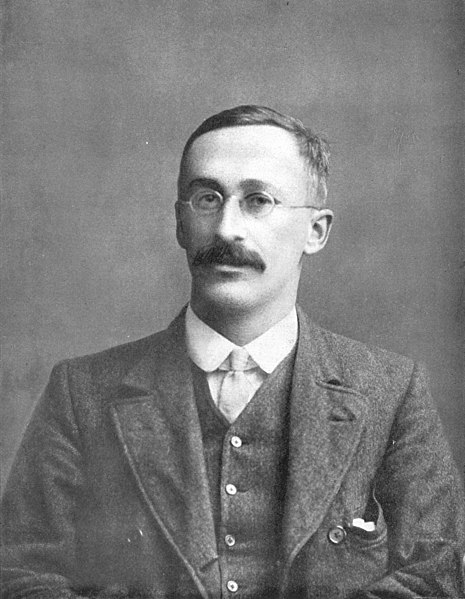
\includegraphics[scale=0.5]{figures/Gosset2.png}\\
%  \vspace{-0.8cm}
%  \caption{William Sealy Gosset, 1908}\label{esquematabela1}}
%\end{figure}


A Guinness era uma empresa de Agro-Química progressista e Gosset iria aplicar os seus conhecimentos de estatística tanto na cervejaria (a destilaria) como nas quintas, para a selecção dos melhores espécimens de cevada.\vskip0.3cm

O trabalho de Gosset na Guinness consistia em medir os inúmeros fatores do processo de produção e ponderar como eles se relacionam aos resultados do produto final. William realizou muitos testes para estimar a duração da cerveja diante das diferentes condições de armazenagem, fabricação e transporte.\vskip0.3cm


Gosset desenvolveu o teste t, distribuição passível de ser tabulada, como um modo barato de monitorar a qualidade da cerveja. Na época, não existia uma teoria para a tomada de decisões com base em pequenas amostras. Por isso, o grande diferencial desse teste é justamente permitir que se façam inferências usando um menor número de elementos. \vskip0.3cm

Um outro funcionário da Guinness tinha já publicado um trabalho que continha alguns segredos da Cervejeira Guinness. Para prevenir fugas de informação e futuras revelações dos "segredos" da marca, a Guinness proibiu que os seus empregados pudessem publicar quaisquer trabalhos independentemente do conteúdo. Isto queria dizer que Gosset não tinha como publicar os trabalhos com o seu nome. Então, usou o pseudonimo $Student$ para as suas publicações evitando ser detectado pela entidade empregadora. \vskip0.3cm

\newpage
Desta forma, o seu feito mais conhecido, é hoje conhecido com a Distribuição t-Student, que noutras circunstâncias seria conhecida como a Distribuição t-Gosset.\vskip0.3cm


Gosset trabalhou na cervejaria em St. James's Gate por 36 anos, antes de se tornar o cervejeiro-chefe de uma nova cervejaria Guinness em Park Royal em Londres.\vskip0.3cm

Em outubro de 2012, uma placa foi inaugurada na Escola Nacional de St Patrick, Blackrock(Irlanda), para homenagear William Sealy Gosset, que morou nas proximidades por 22 anos. \vskip0.3cm

Sir \textbf{Ronald Fisher}, um gigante entre os estatísticos, chamou Gosset de “O Faraday das Estatísticas”, reconhecendo sua capacidade de compreender princípios gerais e aplicá-los a problemas de importância prática.



\subsubsection{A Distribuição $t$ }

Seja a variável aleatória:

\begin{equation}
    t =\frac{\overline{y}-\overline{Y}}{\frac{s(Y)}{\sqrt(n)}}
\end{equation}

Esta variável é conhecida com distribuição $t$ student, com $k=n-1$ graus de liberdade, podendo também ser escrita na forma:

\begin{equation}
    t =\frac{N(0,1)}{\sqrt{\frac{\chi^{2}_{n-1}}{n-1}}}
\end{equation}

O $s(y)$ é considerado o desvio-padrão estimado.\vskip0.3cm

O gráfico da função densidade da variável $t$ de student é simétrico e tem uma forma parecida com a distribuição normal, entretando, menos achatada, com a média zero e variância igual $\frac{k}{(k-2)}$, em que $k>2$ graus de liberdade. A função densidade da variável $t$ é dada pela expressão (2.10). 

\begin{equation}
f\left(t\right)=\frac{1}{\sqrt{k \pi}}\frac{\Gamma\left(\frac{k+1}{2}\right) }{\Gamma \left(\frac{k}{2}\right)}\left(1+\frac{t^2}{k}\right)^{-\left(\frac{\upsilon+1}{2}\right)},~~~-\infty<x<\infty
\end{equation}













\newpage
\subsection{Distribuição F de Snedecor}






A Estatística \textbf{F de Snedecor} é definida como a razão de duas variáveis independentes com distribuição $\chi^{2}$, ou seja:

\begin{equation}
    F_{k,p}=\frac{\frac{\chi^{2}_{k}}{k}}{\frac{\chi^{2}_{p}}{p}}
\end{equation}

O valor $k$ é o número de graus de liberdade do numerador e o $p$ é o número de graus de liberdade do denominador. A função densidade da distribuição F de Snedecor é dada pela Equação (2.9).


 